%%%%%%%%%%%%%%%%%%%%%%%%%%%%%%%%%%%%%%%%%%%%%%%%%%%%%%%%%%%%%%%%%%%%%%%%%%%%%%%%%%%%%%%%%%%
%%%% Die Dokumentenklasse und ihre Optionen %%%%%%%%%%%%%%%%%%%%%%%%%%%%%%%%%%%%%%%%%%%%%%%
\documentclass[captions=tableheading, 12pt, headings=small, parskip=half]{scrartcl}

%%%%%%%%%%%%%%%%%%%%%%%%%%%%%%%%%%%%%%%%%%%%%%%%%%%%%%%%%%%%%%%%%%%%%%%%%%%%%%%%%%%%%%%%%%%
%%%% LaTeX-Pakete %%%%%%%%%%%%%%%%%%%%%%%%%%%%%%%%%%%%%%%%%%%%%%%%%%%%%%%%%%%%%%%%%%%%%%%%%
\usepackage[utf8]{inputenc}
\usepackage[T1]{fontenc}
\usepackage[ngerman]{babel}
\usepackage{setspace,               % Zeilendurchschuss verändern (\doublespacing,\onehalfspacing)
            booktabs,               % Schöne Tabellen
            amsmath,                % Mathepackage der American Mathematical Society
            amsfonts,               % Paket für schönere mathematische Schriftarten
            amssymb,                % Paket für schönere mathematische Symbole
            bbm, 					% Blackboard-Style im Mathemodus
            bm, 					% Bold-Symbols im Mathemodus
            enumitem, 				% Anpassungen der enumerate-Umgebung
            graphicx,               % Paket zum Laden von Graphiken
            lmodern,                % Schrifttyp, der mit Microtype zusammenarbeitet
            nicefrac,				% Schräge Brüche
            csquotes,				% für Anführungszeichen
            microtype,              % Typographische Korrekturen bei Umbrüchen
            hyperref,				% url-Befehl
            calligra,
            setspace,
            multirow,
            float,
            eurosym,
            epstopdf
}
\usepackage[left=2.5cm,right=2.5cm,top=2cm,bottom=2cm]{geometry} % Seiteneinrichtung
%\usepackage{geometry} % Seiteneinrichtung

\usepackage{dcolumn}
\newcolumntype{d}[1]{D{.}{.}{#1}}

% \graphicspath{{C:\Users\stapperm\Documents\Econometrics 1\Code}}



\begin{document}

\begin{table}[H]
	\begin{tabular}{lr}
		& \multirow{4}{*}{
\includegraphics[width = 8cm]{Code1/wwu_logo.png}}\\
		Dr. Willi Mutschler& \\
		M.Sc. Manuel Stapper & \\
		Winter term 2017/2018 \hphantom{MMMMMMMMMMM}& 
	\end{tabular}
\end{table}
\vspace{1cm}
\begin{center}
	{\Large Econometrics I} \\
	-- Exercise Book --
\end{center}

\section*{\underline{Exercise 1}}
Let $A = [a_{ij}]\in\mathbb{R}^{n\times n}$ be a matrix and let $a = (a_1,...,a_n)'$, $x = (x_1,...,x_n)'$, $y = (y_1,...,y_n)'$ be vectors of length $n$.
\begin{enumerate}[label = \alph*)]
	\item Write the sum $\sum_{i=1}^n a_i\cdot x_i$ as a product of vectors.
	\item Write $c_i = \sum_{j=1}^n a_{ij}\cdot x_j$ in matrix form.
	\item Write $\sum_{i=1}^n y_i$ in matrix form. Hint: Use a vector of ones.
	\item Write $\sum_{i=1}^n\sum_{j=1}^n a_{ij}$ in matrix form.
\end{enumerate}

\section*{\underline{Exercise 2}}
Consider the following matrices
\[ A = \left(\begin{array}{d{2.0}d{2.0}d{2.0}}
1 & -1 & 2 \\
3 & 0 & 1 \\
2 & 1 & 0 \\
\end{array}\right),\qquad
B = \left(\begin{array}{c}
1 \\ 2 \\3\\ \end{array}\right),\qquad
C = \left(\begin{array}{d{2.0}d{2.0}d{2.0}}
2 & 0 & 3 \\
7 & -1 & 2 \\
0 & 1 & 1 \\
\end{array}\right)\]

\[ D = \left(\begin{array}{d{2.0}d{2.0}d{2.0}}
2 & 3  \\
-2 & 1 \\
0 & 5 \\
\end{array}\right),\qquad
E = \left(\begin{array}{ccc}
0 & 2 & 1\\
\end{array}\right).
\]
\begin{enumerate}[label = \alph*)]
	\item Calculate (if possible): $AB$, $CD$, $EA$, $BE$, $ED$.
	\item Verify that: $(A+C)' = A' + C'$ and $(AC)'=C'A'$.
\end{enumerate}

\section*{\underline{Exercise 3}}
Consider the following matrices
\[ A= \left(\begin{array}{d{2.0}d{2.0}}
1 & -1 \\
2 & 1 \\
\end{array}\right),\qquad
B= \left(\begin{array}{d{2.0}d{2.0}}
0 & -2 \\
1 & -3 \\
\end{array}\right).\]
\begin{enumerate}[label = \alph*)]
	\item Calculate the determinant of $A$, $B$, $AB$, $A'$, $2A$ and $-B$.
	\item Calculate $A^{-1}$ and $B^{-1}$.
	\item Calculate $(AB)^{-1}$.
	\item Calculate $B^{-1}A^{-1}$ and compare with (b).
	\item Are the matrices $A$ and $C=A'A$ positive definite, negative definite or indefinite?
	\item Give an example of a negative definite and indefinite (2 $\times$ 2) matrix.
\end{enumerate}

\section*{\underline{Exercise 4}}
In this exercise we take a look at an example to understand why the unbiased variance estimator has a factor $\frac{1}{T-1}$ instead of $\frac{1}{T}$. Imagine a box containing 3 coins with values 0, 2 and 4 denoted as $x_1, x_2$ and $x_3$ respectively. Please follow the steps:
\begin{itemize}
	\item Calculate the \textit{population sample} \[\mu := \frac{x_1 + x_2 + x_3}{3}\] and the \textit{population variance} \[\sigma^2 = \frac{1}{3}\sum_{t = 1}^3{(x_t - \mu)^2}\text{ .}\]
	\item We try to estimate the population variance by drawing a coin $T = 2$ times. Write down every combination of two values from the population. Hint: $(0, 2)\ne (2, 0)$
	\item For every of these 9 combinations, calculate the sample average and the sample variance with both factors $\frac{1}{T}$ and $\frac{1}{T-1}$.
	\item Calculate the average of these three key figures over all 9 samples.
	\item What do you notice?
\end{itemize}

\section*{\underline{Exercise 5}}

An investor wants to invest in two possible, independent stocks $A$ and $B$. The return of those two stocks is denoted as $R_A$ and $R_B$. To evaluate the stocks we assume
\[
\operatorname{E}(R_A) = 2 \qquad \operatorname{E}(R_B) = 5 \qquad \operatorname{Var}(R_A) = 2 \qquad \operatorname{Var}(R_B) = 6
\]
\begin{enumerate}[label = \alph*)]
	\item Calculate the expected return in case the investor splits his capital evenly.
	\item Calculate the variance of the above described portfolio. What do you notice?
	\item The investor wants to limit his risk, so that the variance in the portfolio return does not exceed 3.5. What is the maximal return on such a portfolio? How much so you suggest him to invest in $A$ and in $B$?
\end{enumerate}

\section*{\underline{Exercise 6}}
Let $a$ be a column vector of length $n$ and $A$ an ($n\times n$) matrix. For a scalar valued function $f(x)$ of a vector $x$,
\[ \frac{\partial f(x)}{\partial x} = \left[
\begin{array}{c} 
\partial f/\partial x_1\\
\vdots\\
\partial f/\partial x_n\\
\end{array} \right] \]
is called the gradient vector of $f$. For the vector $y = Ax$, define
\[
\frac{\partial y}{\partial x} = \begin{bmatrix}
\partial y_1/\partial x'\\
\partial y_2/\partial x'\\
\vdots\\
\partial y_n/\partial x'
\end{bmatrix}\text{ .}
\]

\begin{enumerate}[label = \alph*)]
	\item Show the following equations:
	\begin{enumerate}[label = \roman*)]
		\item $\frac{\partial a'x}{\partial x} = a$
		\item $\frac{\partial Ax}{\partial x} = A$
		\item $\frac{\partial x'Ax}{\partial x} = (A + A')x$
	\end{enumerate}
	\item What does a) iii) imply for $\frac{\partial x'Ax}{\partial x}$ if $A$ is symmetric?
\end{enumerate}


\section*{\underline{Exercise 7}}

Consider the following linear regression:
\[
y_t = \alpha + \beta x_t + u_t\text{ ,}\qquad\text{ for }t=1,...,T\text{ .}
\]Show that the OLS estimators $\hat{\alpha}$ and $\hat{\beta}$ are given by
\[
\hat{\beta} = \frac{\sum_{t = 1}^T{(x_t - \bar{x})(y_t - \bar{y})}}{\sum_{t = 1}^T{(x_t - \bar{x})^2}}\text{ ,}\qquad \hat{\alpha} = \bar{y} - \hat{\beta}\bar{x}
\]

\section*{\underline{Exercise 8}}

A supermarket chain plans to investigate the connection between marketing expenditure for a certain product and the number of items sold. $T=10$ different but comparable markets are included in the study. For market $t$, marketing expenditure (in USD) and number of items sold are denoted as $x_t$ and $y_t$ respectively.\\
From this study, the following values are calculated:
\begin{align*}
&\bar{x}=1170 \qquad \sqrt{\frac{1}{10}\sum_{t = 1}^{10}{(x_t - \bar{x})^2}} = 415\\
&\sum_{t = 1}^{10}{y_t} = 3500 \qquad \sum_{t = 1}^{10}{y_t^2} = 1'300'000 \qquad \sum_{t = 1}^{10}{x_ty_t} = 4'443'000
\end{align*}
\begin{enumerate}[label = \alph*)]
	\item Calculate the OLS-estimates for $\alpha$ and $\beta$ from the regression model\\
	$y_t = \alpha + \beta x_t + u_t$.
	\item How is $\beta$ interpreted from an economic point of view?
	\item The manager of a market not included in the study wants to sell 500 products, what would you suggest him to spend on marketing?
	\item Calculate the coefficient of determination and interpret it.
\end{enumerate}

\section*{\underline{Exercise 9}}
\begin{enumerate}[label = \alph*)]
	\item State the A-, B- and C-assumptions in your own words.
	\item Give a counterexample of each assumption by drawing a picture if points $(x_t, y_t)$, if possible. Otherwise describe the counterexample in your own words.
\end{enumerate}

\section*{\underline{Exercise 10}}
Take a look at the 6 scatterplots below.
\begin{figure}[H]
	\begin{minipage}{0.32 \columnwidth}
		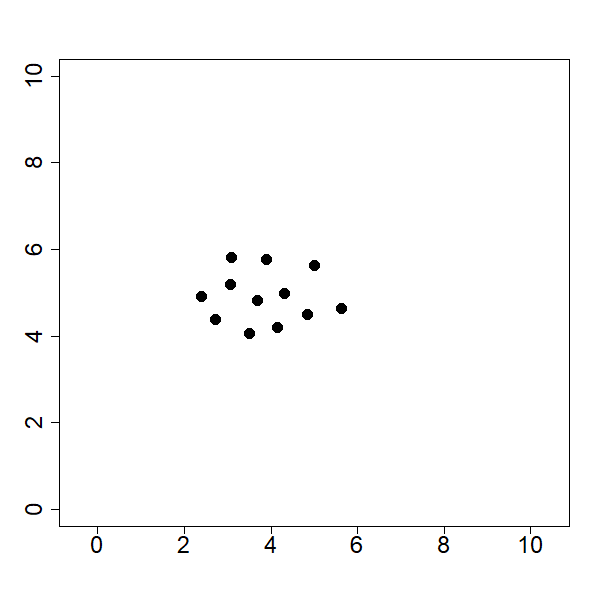
\includegraphics[width = \columnwidth]{Code1/plot1.png}
		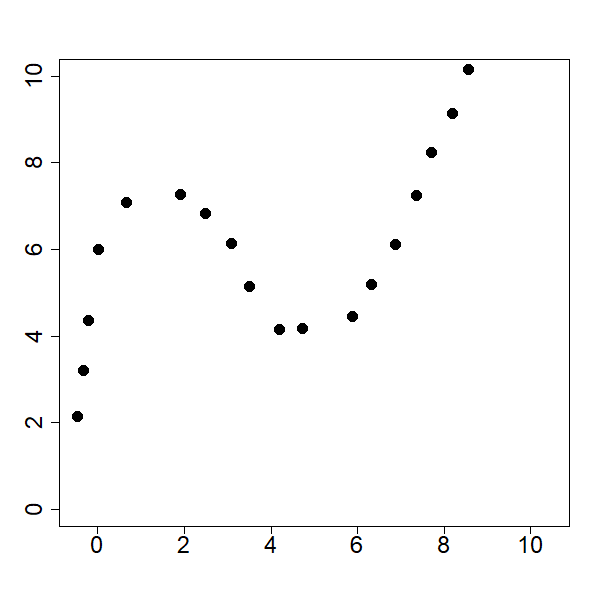
\includegraphics[width = \columnwidth]{Code1/plot4.png}
	\end{minipage}
	\hfill
	\begin{minipage}{0.32 \columnwidth}
		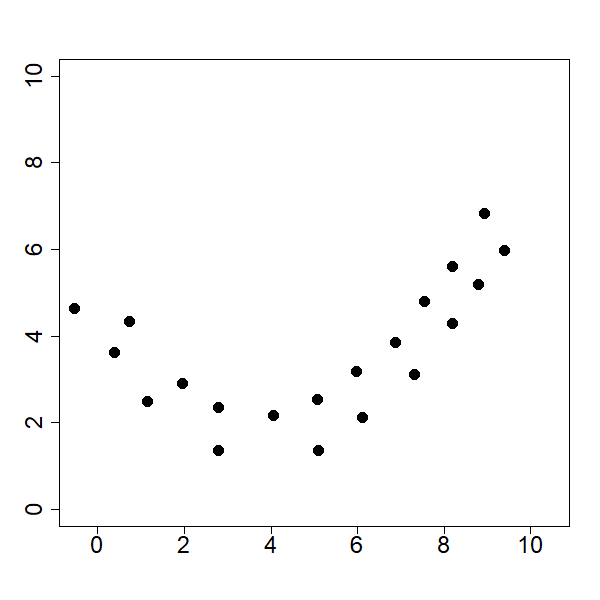
\includegraphics[width = \columnwidth]{Code1/plot2.png}
		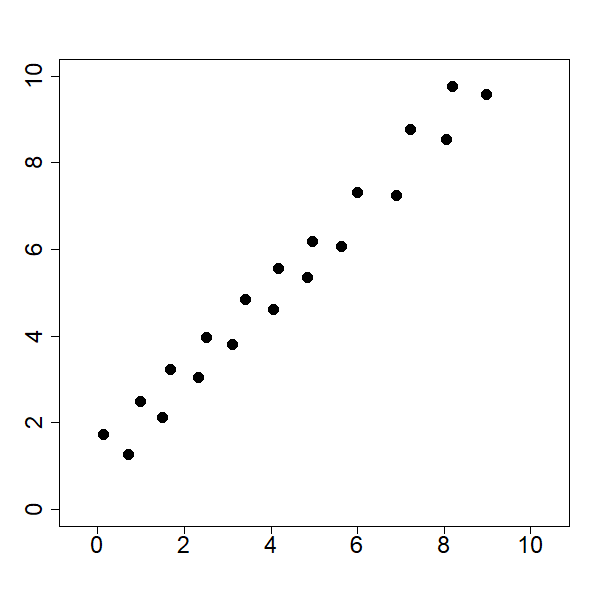
\includegraphics[width = \columnwidth]{Code1/plot5.png}
	\end{minipage}
	\hfill
	\begin{minipage}{0.32 \columnwidth}
		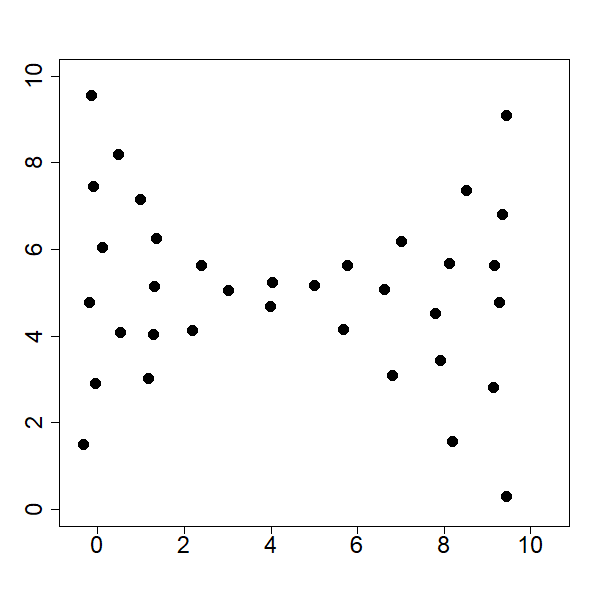
\includegraphics[width = \columnwidth]{Code1/plot3.png}
		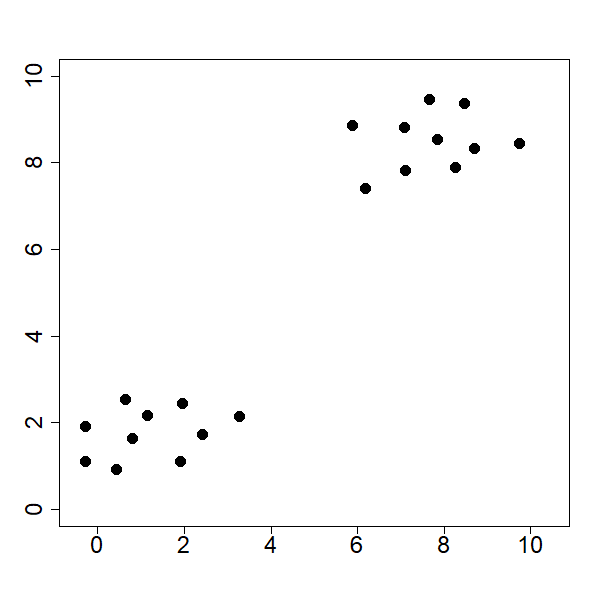
\includegraphics[width = \columnwidth]{Code1/plot6.png}
	\end{minipage}
\end{figure}
\begin{enumerate}[label = \alph*)]
	\item Which of the A-, B- and C-assumptions are not satisfied in the individual cases?
	\item Which of the assumptions could be violated without being visible in a scatterplot?
\end{enumerate}

\section*{\underline{Exercise 11}}
The figure below shows the fitted values of two different regressions $y_t = \alpha + \beta x_t + u_t$. Besides the OLS regression line, the Least Absolute Deviation (LAD) regression line is shown. The LAD-estimators $\tilde{\alpha}$ and $\tilde{\beta}$ are calculated by minimizing
\[
\sum_{t = 1}^{15}{|y_t - (\alpha + \beta x_t)|}\text{ .}
\]
\begin{figure}[h!]
	\begin{minipage}{0.49\columnwidth}
		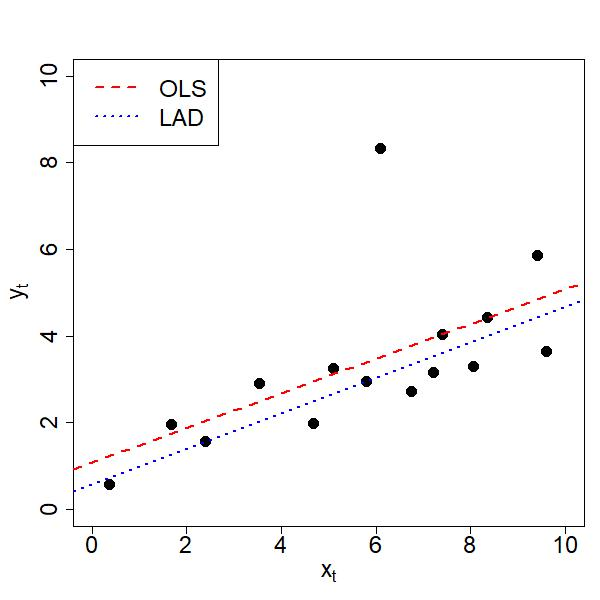
\includegraphics[width = \columnwidth]{Code1/LADreg.jpeg}
	\end{minipage}
	\hfill
	\begin{minipage}{0.49\columnwidth}
		\begin{align*}
		\sum_{t = 1}^{15}{y_t} = 50.67 \quad \sum_{t = 1}^{15}{y_t^2} = 219.53\\
		\sum_{t = 1}^{15}{\hat{y}_t^2} = 188.77 \quad \sum_{t = 1}^{15}{\tilde{y}_t} = 44.16\\
		\sum_{t = 1}^{15}{\tilde{y}_t^2} = 148.48
		\end{align*}
	\end{minipage}
\end{figure}
\begin{enumerate}[label = \alph*)]
	\item Calculate the coefficient of determination $R^2$ for both regressions using the above sums.
	\item Calculate the correlation between $y_t$ and $x_t$.
	\item Interpret the above results.
\end{enumerate}

\section*{\underline{Exercise 12}}
\begin{enumerate}[label = \alph*)]
	\item Consider the regression model \[y_t = \alpha + \beta x_t + u_t\text{ .}\]Is it possible that the coefficient of determination is either negative or larger than 1? Justify your answer briefly.
	\item Consider the regression model \[y_t = \alpha x_t + u_t\text{ .}\]Is it possible that the coefficient of determination is negative or larger than 1? Justify your answer.
\end{enumerate}


\section*{\underline{Exercise 13}}
Consider the following regression:
\[
y_t = \alpha x_t + u_t\text{, \qquad where } u_t\sim \mathcal{N}(0, \sigma^2)
\]for $t = 1,...,T$. Assume validity if all A-, B- and C- assumptions.
\begin{enumerate}[label = \alph*)]
	\item Verify that the OLS estimator $\hat{\alpha}$ satisfies the following relationships
	\[
	\hat{\alpha} = \frac{\sum_{t = 1}^T{x_ty_t}}{\sum_{t = 1}^N{x_t^2}}
	\]and can be represented as
	\[
	\hat{\alpha} = \alpha + \frac{\sum_{t = 1}^T{x_tu_t}}{\sum_{t = 1}^T{x_t^2}} \text{ .}
	\]
	\item Calculate the ML-estimator of $\alpha$.
	\item Verify that the OLS estimator $\hat{\alpha}$ is unbiased for $\alpha$.
	\item Find the distribution of $\hat{\alpha}$.
\end{enumerate}

\section*{\underline{Exercise 14}}

Consider the simple regression model with binary regressor, i.e.
\[y_t = \alpha + \beta x_t + u_t,\qquad x_t\in\{0,1\},\quad y_t\in\mathbb{R}, \quad t = 1,...,T.\]
Let $\bar{y}_A$ and $\bar{y}_B$ denote the mean of $y_t$ for those observations with $x_t = 1$ and  $x_t = 0$ respectively. Further, let $T_A$ denote the number of observations with $x_t = 1$ and correspondingly $T_B = T - T_A$.
\begin{enumerate}[label = \alph*)]
	\item Show that the OLS estimators can be expressed as
	\[
	\hat{\alpha} = \bar{y}_B \qquad \hat{\beta} = \bar{y}_A - \bar{y}_B\text{ .}
	\]
	\item Sketch the above findings in a plot.
	\item What would the OLS estimators be if it wasn't $x_t\in\{0,1\}$, but $x_t\in\{-1,1\}$?
	\item Show that $S_{xx} = \frac{T_AT_B}{T}$ and $(T-2)\hat{\sigma}^2 = S_{yy}^A + S_{yy}^B$, where \[S_{yy}^A = \sum_{A}{(y_t - \bar{y}_A)^2}\qquad \text{and}\qquad S_{yy}^B = \sum_{A}{(y_t - \bar{y}_B)^2}\text{ .}\]
\end{enumerate}
\newpage


\section*{\underline{Exercise 15}}
A supermarket chain is interested in the effect of bonus scheme on the profit. The 35 stores in the suburbs offer the bonus scheme, while the 25 stores in the city do not use it. The following table summarizes the results of a study:
\begin{table}[h!]
	\centering
	\begin{tabular}{ccc}
		\toprule
		\toprule
		&No bonus scheme & Bonus scheme\\
		\midrule
		Number of Stores&25&35\\
		Mean Return&117.58&122.46\\
		Sum of squared Returns&347686&527799\\
		\bottomrule
		\bottomrule
	\end{tabular}
\end{table}
\begin{enumerate}[label = \alph*)]
	\item What model would be suitable to investigate the effect of the bonus scheme on the return?
	\item Estimate the parameters of the above suggested model and interpret them.
	\item Calculate 95\% confidence intervals for the above estimates. (table of quantiles attached)
	\item The CEO of the chain asks, if you suggest to introduce the bonus scheme to the stores in the city based on the data. What do you reply?
\end{enumerate}

\section*{\underline{Exercise 16}}
The following table displays the results of a study with allergy patients. We investigate the effect of medication (Dosage $x_t$) on the time of relief $y_t$ by assuming the model $y_t = \alpha + \beta x_t + u_t$. 
\begin{figure}[H]
	\begin{minipage}{0.51 \columnwidth}
		\begin{tabular}{ccccc}
			\toprule
			\toprule
			&$x_t$ &$y_t$&$x_ty_t$&$\hat{y}_t$\\
			\midrule
			&3&9&27&7.15\\
			&3&5&15&7.15\\
			&4&12&48&9.89\\
			&5&9&45&12.63\\
			&6&14&84&15.37\\
			&6&16&96&15.37\\
			&7&22&154&18.11\\
			&8&18&144&20.86\\
			&8&24&192&20.86\\
			&9&22&198&23.60\\
			\midrule
			$\Sigma$&59&151&1003&151\\
			SSQ\footnote[1]{ SSQ: Sum of squared values - SSQ($x$) = $\sum x_t^2$\\Not the same as $S_{xx}$}&389&2651&--&2587.35\\
			\bottomrule
			\bottomrule
		\end{tabular}
	\end{minipage}
	\hfill
	\begin{minipage}{0.48\columnwidth}
		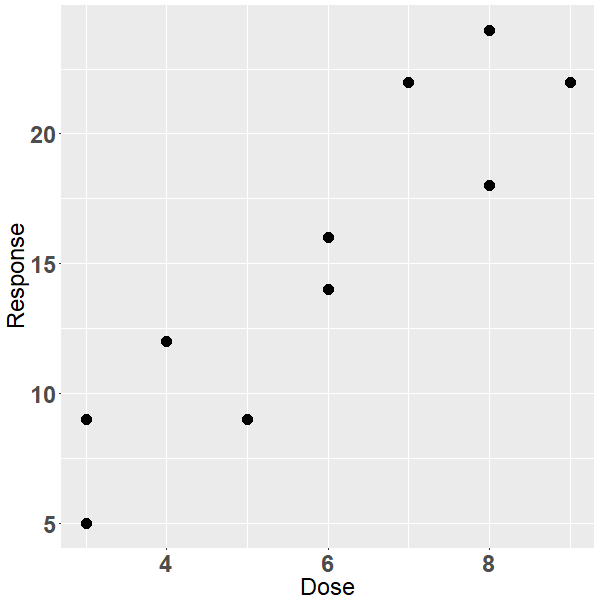
\includegraphics[width = \columnwidth]{Code1/DoseResp.png}
	\end{minipage}
\end{figure}
\begin{enumerate}[label = \alph*)]
	\item Are the assumptions satisfied?
	\item Estimate the parameters $\alpha$ and $\beta$ by OLS.
	\item Calculate the 95\% confidence intervals for $\hat{\alpha}$ and $\hat{\beta}$ and interpret.
	\item The following figure shows the 95\% confidence interval around the regression line. Try to think of a reason why the this confidence band is wider at the edges.
	\begin{figure}[H]
		\centering
		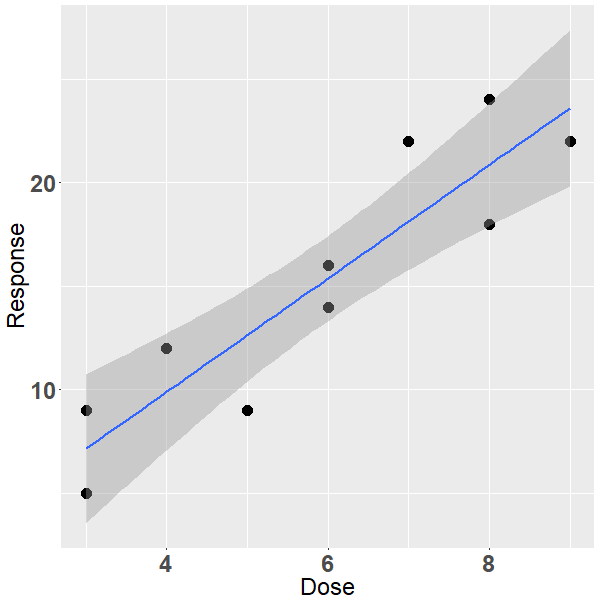
\includegraphics[width = 0.5\columnwidth]{Code1/DoseRespFit.png}
	\end{figure}
\end{enumerate}


\section*{\underline{Exercise 17}}
Consider the regression model $y_t = \alpha + \beta x_t + u_t$. Show that $\hat{\sigma}^2 = \frac{1}{T-2}\sum_{t=1}^T \hat{u}_t^2$ is an unbiased estimator of the variance of the error terms by following the steps:
\begin{enumerate}[label = Step \arabic*)]
	\item Show that $y_t - \bar{y} = \beta(x_t - \bar{x}) + (u_t - \bar{u})$
	\item Show that $\hat{\beta} = \beta + \frac{S_{xu}}{S_{xx}}$.
	\item Show that $\hat{u}_t = (y_t - \bar{y}) - \hat{\beta}(x_t - \bar{x}) = -(\hat{\beta} - \beta)(x_t - \bar{x}) + u_t - \bar{u}$
	\item Conclude that $\sum_{t = 1}^T{\hat{u}_t^2} = S_{uu} -(\hat{\beta}-\beta)^2S_{xx}$
	\item Show that E$(S_{uu}) = (T-1)\sigma^2$
	\item Show that E$\left((\hat{\beta} - \beta)^2\right)S_{xx} = \sigma^2$ which finishes the proof
\end{enumerate}
\newpage
\section*{\underline{Exercise 18}}
This exercise deals with multicollinearity. As a reminder, consider a regression model $y_t = \beta_0 + \beta_1 x_{1, t} + ... + \beta_k x_{k, t} + u_t$. Multicollinearity exists if there is a vector $\gamma = (\gamma_0, ..., \gamma_k)'\ne (0,...,0)'$ so that $\gamma_0 + \gamma_1 x_{1,t} + ... + \gamma_k x_{k, t} = 0$ for every $t = 1,...,T$. \\
\begin{enumerate}[label = \alph*)]
	\item Are the following statements true or false?
	\begin{enumerate}[label = (\roman*)]
		\item In case of multicollinearity, at least one exogenous variable can be expressed as a linear combination of the remaining ones.
		\item If $y_t$ can be expressed as linear combination of the exogenous variables $x_{1,t},...,x_{k,t}$, the OLS estimator can not be calculated.
		\item To check if multicollinearity is in the data, it suffices to calculate the pairwise correlation coefficients of exogenous variables.
		\item In case two exogenous variables are perfectly correlated, i.e. $x_{1,t} = \gamma_0 + \gamma_1 x_{2,t}$, the total impact of those variables on $y_t$ can be estimated.\\
		If yes, can the impact be separated on the two variables?\\
		If no, can you think of a way to solve the problem?
		\item In case of multicollinearity, the determinant of $X'X$ is 0.
	\end{enumerate}
\item Decide if there is multicollinearity in the cases below:
\begin{enumerate}[label = (\roman*)]
	\item Model: $y_t = \beta_0 + \beta_1x_t + u_t$\\
	$S_{xx} = \sum_{t = 1}^T{(x_i - \bar{x})^2} = 0$
	\item Model: $y_t = \beta_0 + \beta_1 x_{1,t} + \beta_2 x_{2,t} + \beta_3 x_{3,t} + u_t$
	\begin{figure}[h!]
	\begin{minipage}{0.49\columnwidth}
	\begin{table}[H]
	\centering
	\begin{tabular}{llll}
	\toprule
	\toprule
	$t$&$x_{1,t}$&$x_{2,t}$&$x_{3,t}$\\
	\midrule
	1 & 2 & 1 & 12 \\ 
	2 & 2 & 1 & 12 \\ 
	3 & 3 & 3 & 9 \\ 
	4 & 5 & 1 & 9 \\ 
	5 & 2 & 3 & 10 \\ 
	6 & 5 & 2 & 8 \\ 
	7 & 6 & 3 & 6 \\ 
	8 & 4 & 6 & 5 \\ 
	9 & 3 & 1 & 11 \\ 
	10 & 1 & 3 & 11 \\
	\midrule
	$\sum_{t = 1}^{10}{x_{\bullet t}}$ &33&24&93\\
	$\sum_{t = 1}^{10}{x_{\bullet t}^2}$ &133&80&917\\
	\bottomrule
	\bottomrule  
\end{tabular}
\end{table}
\end{minipage}
\hfill
\begin{minipage}{0.49\columnwidth}
	\begin{align*}
	\sum_{t = 1}^{10}{x_{1,t}x_{2,t}} &= 82\\
	\sum_{t = 1}^{10}{x_{1,t}x_{3,t}} &= 280\\
	\sum_{t = 1}^{10}{x_{2,t}x_{3,t}} &= 198\\
	\end{align*}
\end{minipage}
\end{figure}
\end{enumerate}
\end{enumerate}
\newpage
\section*{\underline{Exercise 19}}
Consider the restricted regression
\[
y_t = \alpha + u_t\text{ , }t = 1,...,T\text{ ,}
\]for which the A-, B- and C-assumption are satisfied.
\begin{enumerate}[label = \alph*)]
	\item Derive the ML estimator for $\alpha$.
	\item Calculate the ML estimator for the error variance given the sample
	\begin{table}[H]
		\centering
		\begin{tabular}{c|cccc}
			\toprule
			$y_t$ & 4&6&7&4\\
			\midrule
			$x_t$ & 2&4&5&3\\
			\bottomrule
		\end{tabular}
	\end{table}
\end{enumerate}


\section*{\underline{Exercise 20}}
Reconsider exercise 8.
\begin{enumerate}[label = \alph*)]
	\item Test if $\beta$ is significantly different from 0 at a 5\% level and interpret the outcome.
	\item Is the intercept $\alpha$ significantly greater than 1? (Choose a 5\% level of significance)\\
	Hint: $\text{Var}\left(\hat{\alpha}\right) = \sigma^2\left[\frac{1}{T} + \frac{\bar{x}^2}{\sum_{t = 1}^T{(x_t - \bar{x})^2}}\right]$
\end{enumerate}

\section*{\underline{Exercise 21}}
It is known that the IQ is normally distributed with mean $\mu = 100$ and standard deviation $\sigma = 15$. Four students want to find out if students have a significantly higher IQ. Therefore they do an IQ test, in which they scored 120 on average. 
\begin{enumerate}[label = \alph*)]
	\item Formulate the hypotheses for above question.
	\item We want to use the average score of 120 as a test statistics. Find the critical value for testing with a 5\% level of significance.\\
	Hint: Use the 95\% quantile of the $\mathcal{N}(0,1)$ distribution $1.645$.
	\item Below figure shows the densities of the average score if $H_0$ was true (black) and the estimated density from the sample (red). Complete the plot by adding
	\begin{enumerate}[label = (\roman*)]
		\item The critical value
		\item The type I error
		\item The type II error if the IQ of students is really 120 on average
	\end{enumerate}
\begin{figure}[H]
	\centering
	\includegraphics[height = \columnwidth, angle = -90]{Code1/IQ.eps}
\end{figure}
	\item Sketch what happens with type I and type II error if the level of significance is increased. Use below figure again.
	\begin{figure}[H]
		\centering
		\includegraphics[height = \columnwidth, angle = -90]{Code1/IQ.eps}
	\end{figure}
\end{enumerate}

\section*{\underline{Exercise 22}}
The following plots show possible density functions of test statistics and critical values. If it belongs to a valid test, give the hypotheses and the level of significance.
\begin{figure}[H]
	\begin{minipage}{0.49\columnwidth}
		\includegraphics[height = \columnwidth, angle = -90]{Code1/CV1.eps}
		\includegraphics[height = \columnwidth, angle = -90]{Code1/CV2.eps}
	\end{minipage}
\hfill
	\begin{minipage}{0.49\columnwidth}
		\includegraphics[height = \columnwidth, angle = -90]{Code1/CV3.eps}
		\includegraphics[height = \columnwidth, angle = -90]{Code1/CV4.eps}
	\end{minipage}
\end{figure}

\section*{\underline{Exercise 23}}
For the annual turnover of a large store group, the validity of the following linear regression model is assumed:
\[
y_t = \alpha + \beta_1x_{1,t} + \beta_2x_{2,t} + u_t
\]with $y_t$: annual turnover (of store $t$), $x_{1,t}$: sales area (of store $t$), $x_{2,t}$: average frequency of people passing by (of store $t$), $u_t$: error term (of store $t$). Based on the observation values collected in $\boldsymbol{y}$ and $\boldsymbol{X}$ one obtains
\[
\boldsymbol{X}'\boldsymbol{X} =
\begin{pmatrix}
20 & 200 & 0 \\
200 & 2014.4 & 16 \\
0 & 16 & 40
\end{pmatrix} \text{ ,}\qquad
(\boldsymbol{X}'\boldsymbol{X})^{-1} = 
\begin{pmatrix}
12.55 & -1.25 & 0.5 \\
-1.25 & 0.125 & -0.05 \\
0.5 & -0.05 & 0.045
\end{pmatrix}\text{ ,}
\]
\[
\boldsymbol{X}'\boldsymbol{y} = \begin{pmatrix} 946\\9532\\85 \end{pmatrix}\text{ ,} \qquad
\boldsymbol{\hat{u}}'\boldsymbol{\hat{u}} = 90.28125\text{ .}
\]
\begin{enumerate}[label = \alph*)]
	\item How many stores were involved in the investigation?
	\item Find the OLS estimators of $\alpha$, $\beta_1$ and $\beta_2$.
	\item Test the null hypothesis that coefficients associated with the regressors $x_{1,t}$ and $x_{2,t}$ are equal at a 5\% level of significance.
\end{enumerate}


\section*{\underline{Exercise 24}}
Consider a dataset with 500 observations of the variables $y, x_1,x_2,x_3$ and the specification
\[
y_t = \alpha + \beta_1x_{1,t} + \beta_2x_{2,t} + \beta_3x_{3,t} + u_t
\]under the validity of A-, B- and C-assumptions. The following values are given
\[
\hat{\boldsymbol{u}}'\hat{\boldsymbol{u}} = 2912.778\text{ ,}\qquad \hat{\boldsymbol{\beta}} =\left(\begin{array}{d{2.2}}
10.85\\2.14\\-0.28\\9.53
\end{array}\right)
\]
\[
(\boldsymbol{X}'\boldsymbol{X})^{-1}=\left(\begin{array}{d{2.4}d{2.4}d{2.4}d{2.4}}
0.0229&-0.0020&-0.0005&-0.0060\\
-0.0020&0.0020&-0.0001&0.0001\\
-0.0005&-0.0001&0.0031&-0.0019\\
-0.0060&0.0001&-0.0019&0.0033
\end{array}\right)\text{ .}
\]
\begin{enumerate}[label = \alph*)]
	\item Test $H_0:\beta_2 = 3$ vs. $H_1: \beta_2 \ne 3$.\\
\end{enumerate}
After your preliminary analysis you find an additional observed variable $x_4$ and may want to include it in your specification.
	\[
	y_t = \alpha + \beta_1x_{1,t} + \beta_2x_{2,t} + \beta_3x_{3,t} + \beta_4x_{4,t} + u_t\text{ .}
	\]The values for the new specification are given by
	\[
	\hat{\boldsymbol{u}}'\hat{\boldsymbol{u}} = 117.138\text{ ,}\qquad \hat{\boldsymbol{\beta}} =\left(\begin{array}{d{1.3}d{1.3}d{1.3}d{1.3}d{1.3}d{1.3}}
	1.061&1.965&2.967&4.040&4.986
	\end{array}\right)'
	\]
	\[
	(\boldsymbol{X}'\boldsymbol{X})^{-1}=\left(\begin{array}{d{2.4}d{2.4}d{2.4}d{2.4}d{2.4}}
	0.0572&-0.0014&-0.0119&0.0132&-0.0175\\
	-0.0014&0.0020&-0.0003&0.0004&-0.0003\\
	-0.0119&-0.0003&0.0069&-0.0083&0.0058\\
	0.0132&0.0004&-0.0083&0.0141&-0.0098\\
	-0.0175&-0.0003&0.0058&-0.0098&0.0089
	\end{array}\right)\text{ .}
	\]
\begin{enumerate}[label = \alph*)]
\setcounter{enumi}{1}
	\item Test $H_0: \beta_2 = 3$ vs. $H_1: \beta_2\ne 3$.
	\item How would you explain the difference in the results from a) and b)?
	\item Can you be sure that your result from b) is valid?
\end{enumerate}


\section*{\underline{Exercise 25}}

Consider a regression model $y_t = \alpha + \beta x_t + u_t$. The parameters are estimated by OLS and the following sums are obtained:
\[
\sum_{t = 1}^{15}{y_t} = 63.8808 \qquad \sum_{t = 1}^{15}{y_t^2} = 289.9335 \qquad \sum_{t = 1}^{15}{\hat{y}_t^2} = 272.1864
\]
\begin{enumerate}[label = \alph*)]
	\item Calculate the adjusted coefficient of determination
	\[
	\bar{R}^2 = 1 - \frac{\frac{1}{T-k-1} \sum_{t = 1}^T{(y_t - \hat{y}_t)^2}}{\frac{1}{T-1} \sum_{t = 1}^T{(y_t - \bar{y})^2}}
	\]
	\item The observations are displayed in the figure below. How do you explain the results in a)?
	\begin{figure}[H]
		\centering
		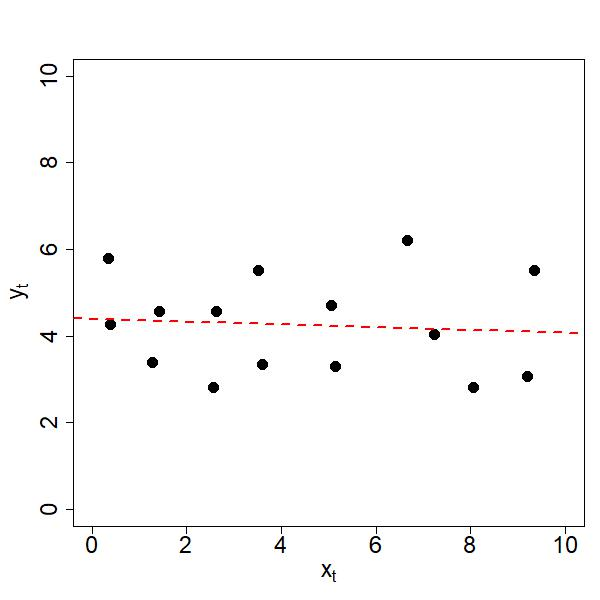
\includegraphics[width = 0.5\columnwidth]{Code1/negR.jpeg}
	\end{figure}
\end{enumerate}

\section*{\underline{Exercise 26}}

Consider the multivariate linear regression model $y = X\beta + u$. The exogenous variables summarized in matrix $X$ were assumed to be non-stochastic. That is not plausible in many economic applications. For this exercise we replace the assumption "'$X$ is not stochastic"' by the two assumptions $\operatorname{E}(u|X)=0$ and $\operatorname{Var}(u|X) = \sigma^2I_T$, where $I_T$ is the identity matrix of dimension $T\times T$.\\
For the following proofs you can use the \textit{law of iterated expectation} and the \textit{law of total variance}. For two random variables $X$ and $Y$ they are defied as:
\begin{align*}
	\operatorname{E}(X) &= \operatorname{E}\left[\operatorname{E}\left(X|Y\right)\right]\\
	\operatorname{Var}(X) &= \operatorname{Var}\left[\operatorname{E}\left(X|Y\right)\right] + \operatorname{E}\left[\operatorname{Var}\left(X|Y\right)\right]
\end{align*}
\begin{enumerate}[label = \alph*)]
	\item Show that the OLS estimator $\hat{\beta} = (X'X)^{-1}X'y$ is unbiased for $\beta$.
	\item Derive the variance of the OLS estimator $\hat{\beta}$.
\end{enumerate}

\newpage
\section*{\underline{Exercise 27}}
Consider the multivariate linear regression model $y = X\beta + u$ with $K = 3$ exogenous variables and an intercept. How would you test the following hypotheses? Translate the hypotheses to the notation $\quad R\text{ }\beta (\ge/ = / \le)\text{ }q \quad$ and sketch the steps to find the test decision if possible.
\begin{enumerate}[label = \alph*)]
	\item $H_0: \beta_1 = \beta_2 = \beta_3 = 0$
	\item $H_0: \beta_1 = \beta_2 = \beta_3$
	\item $H_0: \beta_1 = 2\beta_2 = 3\beta_3$
	\item $H_0: \frac{\beta_0}{\beta_1} = 2$
	\item $H_0: \beta_1 \ge \beta_2$
\end{enumerate}

\section*{\underline{Exercise 28}}
To estimate the consumption function for the years 1962 to 2001, the regression model
\[y_t = \beta_0 + \beta_1x_{1,t} + \beta_2x_{2,t} + u_t\]
is considered with
\begin{align*}
	y_t&: \text{Consumption}\\
	x_{1,t} &: \text{Income}\\
	X_{2,t} &: \text{Interest rate.}
\end{align*}The following results are obtained:
\[X'X = \begin{pmatrix}40&0&10\\0&100&10\\10&10&20\end{pmatrix}\]
The OLS estimators were first calculated without the variable $x_{2,t}$.
\begin{enumerate}[label = \alph*)]
	\item On what condition are $\hat{\beta}_0$ and $\hat{\beta}_1$ unbiased?
	\item Is there an omitted variable bias?
	\item Calculate the bias $\operatorname{E}(\hat{\beta}_0) - \beta_0$ and $\operatorname{E}(\hat{\beta}_1) - \beta_1$ by assuming $\beta_2 = -0.1$.
	\item Assuming that there is no omitted variable bias. What consequences would if expect when adding $x_{2,t}$ to the model?
\end{enumerate}


\section*{\underline{Exercise 29}}

A friend had asked you to do a regression for his master's thesis. For the model
\[
y_t = \alpha + \beta x_t + u_t\qquad t = 1,...,T
\]you estimated the parameters given the following information
\[
	\sum x_t = 19.3 \qquad \sum x_t^2 = 47.16  \qquad \sum x_ty_t = 654.4 \]\[\sum y_t =272.48  \qquad \sum y_t^2 = 9223.33  \qquad \bar{x} = 1.93 \]
After speaking to his professor, your friends tells you about two problems. First, he omitted a relevant variable and, second, $x_t$ has a quadratic impact on $y_t$.
\begin{enumerate}[label = \alph*)]
	\item Your friend asks you why you did not tell him about these problems. Was it possible for you to recognize them without further information about the theoretical background of the data?
	\item Which assumptions are violated by the described problems and what are the consequences?
	\item Consider the model $y_t = \alpha + \beta_1 x_{1,t} + \beta_2 x_{2,t} + u_t$ where $x_{2,t} = x_t^2$. Assume that the A-, B- and C-assumptions hold. Calculate the OLS esimator.\\
	First calculations provide the following results. 
	\begin{equation*}
	\begin{array}{cc}
	X=%
	\begin{pmatrix}
	1 & 7.02 & 0.10 \\ 
	1 & 5.76 & 0.30 \\ 
	1 & 9.61 & 0.39 \\ 
	1 & 1.21 & 0.41 \\ 
	1 & 4.41 & 0.26 \\ 
	1 & 0.00 & 0.11 \\ 
	1 & 8.70 & 0.55 \\ 
	1 & 7.02 & 0.63 \\ 
	1 & 0.36 & 0.36 \\ 
	1 & 3.06 & 0.27%
	\end{pmatrix}
	& y=%
	\begin{pmatrix}
	35.22 \\ 
	31.12 \\ 
	47.76 \\ 
	13.52 \\ 
	25.73 \\ 
	8.28 \\ 
	44.24 \\ 
	36.99 \\ 
	9.52 \\ 
	20.11%
	\end{pmatrix}
	\\ 
	X^{\prime }X=%
	\begin{pmatrix}
	10.00 & 47.15 & 3.38 \\ 
	47.15 & 330.19 & 17.98 \\ 
	3.38 & 17.98 & 1.40%
	\end{pmatrix}
	& (X^{\prime }X)^{-1}=%
	\begin{pmatrix}
	0.59 & -0.02 & -1.13 \\ 
	-0.02 & 0.01 & -0.09 \\ 
	-1.13 & -0.09 & 4.54%
	\end{pmatrix}
	\\ 
	X^{\prime }y=%
	\begin{pmatrix}
	272.49 \\ 
	1724.82 \\ 
	101.12%
	\end{pmatrix}
	& My=%
	\begin{pmatrix}
	-0.58 \\ 
	-0.22 \\ 
	0.67 \\ 
	0.15 \\ 
	-0.06 \\ 
	0.68 \\ 
	0.32 \\ 
	-0.41 \\ 
	-0.28 \\ 
	-0.28%
	\end{pmatrix}%
	\end{array}%
	\end{equation*}
	\item Your friend believes that $\beta _{1}=\beta _{2}$ and, in
	addition, $\alpha =\beta _{1}+\beta _{2}$. Test his hypothesis with one of
	the tests discussed in the lecture.
\end{enumerate}

\section*{\underline{Exercise 30}}
At the football world cup 2010 in South Africa, the atmosphere at match $t$ ($y_t$) was measured by a rating system. To model it, the regression model
\[y_t = \beta_0 + \beta_1x_t + u_t\]
is assumed, where $x_t$ is the number of vuvuzelas (in 10 thousand). The following results were obtained from the study
\[
	X'X= \begin{pmatrix}
	64&288.128\\288.128&1842.3374
	\end{pmatrix}\qquad (X'X)^{-1} = \begin{pmatrix}
	0.0528&-0.0083\\-0.0083&0.0018
	\end{pmatrix}
\]\[
	X'y = \begin{pmatrix}
	6080\\27496
	\end{pmatrix}
\]
\begin{enumerate}[label = \alph*)]
	\item Calculate the OLS estimator.
	\item Calculate the coefficient of determination under the assumption $y'y = 577700$.
	\item Give a prognosis for the atmosphere rating if $x_0 = 3$.
	\item Conduct a 95\% prognosis interval for $y_0$ with $x_0 = 3$. Thereby assume an error variance $\hat{\sigma}^2 = 1$.
\end{enumerate}

\section*{\underline{Exercise 31}}
Explain the idea behind Wald-, LR- and LM-test by summarizing the idea in two sentences and completing the images.
\begin{enumerate}[label = \alph*)]
	\item Wald-test
	\begin{figure}[H]
		\centering
		\includegraphics[height = 0.75\columnwidth, angle = -90]{Code1/Gamma_Wald_LR.eps}
	\end{figure}
	\item LR-test
\begin{figure}[H]
	\centering
	\includegraphics[height = 0.75\columnwidth, angle = -90]{Code1/Gamma_Wald_LR.eps}
\end{figure}
	\item LM-test
\begin{figure}[H]
	\centering
	\includegraphics[height = 0.75\columnwidth, angle = -90]{Code1/Gamma_LM.eps}
\end{figure}
\end{enumerate}

\newpage
\section*{\underline{Exercise 32}}
The \textit{International Monetary Found} hires you to estimate the credit demand function for the private sector
\[
	y_t = \alpha + \beta x_t + u_t\qquad t = 1,...,T
\]based on a sample of $T = 40$ countries. Thereby $y_t$ gives the total of private credits in country $t$ (in billion USD) and $x_t$ the average nominal interest rate in country $t$ (in percent). Further you get the following values:
\[
	\sum_{t = 1}^T{x_t} = 250; \quad \sum_{t = 1}^T{x_t^2} = 1600; \quad \sum_{t = 1}^T{y_t} = 200; \quad
\sum_{t = 1}^T{y_t^2}=1015.78; \quad \sum_{t = 1}^T{x_ty_t} = 1227.5
\]
\begin{enumerate}[label = \alph*)]
	\item Estimate the coefficients $\alpha$ and $\beta$ by OLS and interpret.
	\item Calculate and interpret the coefficient of determination $R^2$.
	\item Estimate the error variance $\sigma^2 = \textrm{Var}(u_t)$.
	\item Test if the impact of nominal interest rate on the total of private credits is significantly different from zero.
	\item Give a prognosis for a country with a nominal interest rate of $x_0 = 3$ (percent) and construct the 95\% prognosis interval. 
\end{enumerate}

\section*{\underline{Exercise 33}}
Consider a multivariate linear regression model $y = X\beta + u$. Show that the estimator $\hat{\beta}^* = (X'BX)^{-1}X'By$ is unbiased. The matrix $B$ is not stochastic, of suitable dimension and chosen so that the inverse $X'BX$ exists.



\newpage
\begin{table}[ht]
	\centering
	\resizebox{\columnwidth}{!}{\begin{tabular}{>{\bfseries}rd{1.3}d{1.3}d{1.3}d{2.3}d{2.3}|>{\bfseries}rd{1.3}d{1.3}d{1.3}d{2.3}d{2.3}}
			\toprule
			\toprule
			df  & \multicolumn{1}{c}{90\%} & \multicolumn{1}{c}{92.5\%} & \multicolumn{1}{c}{95\%} & \multicolumn{1}{c}{97.5\%} & \multicolumn{1}{c}{99\%} & df  & \multicolumn{1}{c}{90\%} & \multicolumn{1}{c}{92.5\%} & \multicolumn{1}{c}{95\%} & \multicolumn{1}{c}{97.5\%} & \multicolumn{1}{c}{99\%} \\
			\midrule
			1 & 3.078 & 4.165 & 6.314 & 12.706 & 31.821 &  51 & 1.298 & 1.462 & 1.675 & 2.008 & 2.402  \\ 
			2 & 1.886 & 2.282 & 2.920 & 4.303 & 6.965 &  52 & 1.298 & 1.461 & 1.675 & 2.007 & 2.400   \\ 
			3 & 1.638 & 1.924 & 2.353 & 3.182 & 4.541 &  53 & 1.298 & 1.461 & 1.674 & 2.006 & 2.399   \\ 
			4 & 1.533 & 1.778 & 2.132 & 2.776 & 3.747 & 54 & 1.297 & 1.460 & 1.674 & 2.005 & 2.397  \\ 
			5 & 1.476 & 1.699 & 2.015 & 2.571 & 3.365 & 55 & 1.297 & 1.460 & 1.673 & 2.004 & 2.396   \\ 
			6 & 1.440 & 1.650 & 1.943 & 2.447 & 3.143 & 56 & 1.297 & 1.460 & 1.673 & 2.003 & 2.395   \\ 
			7 & 1.415 & 1.617 & 1.895 & 2.365 & 2.998 & 57 & 1.297 & 1.459 & 1.672 & 2.002 & 2.394   \\ 
			8 & 1.397 & 1.592 & 1.860 & 2.306 & 2.896 & 58 & 1.296 & 1.459 & 1.672 & 2.002 & 2.392  \\ 
			9 & 1.383 & 1.574 & 1.833 & 2.262 & 2.821 & 59 & 1.296 & 1.459 & 1.671 & 2.001 & 2.391   \\ 
			10 & 1.372 & 1.559 & 1.812 & 2.228 & 2.764 & 60 & 1.296 & 1.458 & 1.671 & 2.000 & 2.390   \\ 
			11 & 1.363 & 1.548 & 1.796 & 2.201 & 2.718 & 61 & 1.296 & 1.458 & 1.670 & 2.000 & 2.389   \\ 
			12 & 1.356 & 1.538 & 1.782 & 2.179 & 2.681 & 62 & 1.295 & 1.458 & 1.670 & 1.999 & 2.388   \\ 
			13 & 1.350 & 1.530 & 1.771 & 2.160 & 2.650 & 63 & 1.295 & 1.457 & 1.669 & 1.998 & 2.387   \\ 
			14 & 1.345 & 1.523 & 1.761 & 2.145 & 2.624 & 64 & 1.295 & 1.457 & 1.669 & 1.998 & 2.386   \\ 
			15 & 1.341 & 1.517 & 1.753 & 2.131 & 2.602 & 65 & 1.295 & 1.457 & 1.669 & 1.997 & 2.385   \\ 
			16 & 1.337 & 1.512 & 1.746 & 2.120 & 2.583 & 66 & 1.295 & 1.456 & 1.668 & 1.997 & 2.384  \\ 
			17 & 1.333 & 1.508 & 1.740 & 2.110 & 2.567 & 67 & 1.294 & 1.456 & 1.668 & 1.996 & 2.383  \\ 
			18 & 1.330 & 1.504 & 1.734 & 2.101 & 2.552 & 68 & 1.294 & 1.456 & 1.668 & 1.995 & 2.382   \\ 
			19 & 1.328 & 1.500 & 1.729 & 2.093 & 2.539 & 69 & 1.294 & 1.456 & 1.667 & 1.995 & 2.382  \\ 
			20 & 1.325 & 1.497 & 1.725 & 2.086 & 2.528 & 70 & 1.294 & 1.456 & 1.667 & 1.994 & 2.381  \\ 
			21 & 1.323 & 1.494 & 1.721 & 2.080 & 2.518 & 71 & 1.294 & 1.455 & 1.667 & 1.994 & 2.380  \\ 
			22 & 1.321 & 1.492 & 1.717 & 2.074 & 2.508 & 72 & 1.293 & 1.455 & 1.666 & 1.993 & 2.379   \\ 
			23 & 1.319 & 1.489 & 1.714 & 2.069 & 2.500 & 73 & 1.293 & 1.455 & 1.666 & 1.993 & 2.379   \\ 
			24 & 1.318 & 1.487 & 1.711 & 2.064 & 2.492 & 74 & 1.293 & 1.455 & 1.666 & 1.993 & 2.378   \\ 
			25 & 1.316 & 1.485 & 1.708 & 2.060 & 2.485 & 75 & 1.293 & 1.454 & 1.665 & 1.992 & 2.377  \\ 
			26 & 1.315 & 1.483 & 1.706 & 2.056 & 2.479 & 76 & 1.293 & 1.454 & 1.665 & 1.992 & 2.376   \\ 
			27 & 1.314 & 1.482 & 1.703 & 2.052 & 2.473 & 77 & 1.293 & 1.454 & 1.665 & 1.991 & 2.376   \\ 
			28 & 1.313 & 1.480 & 1.701 & 2.048 & 2.467 & 78 & 1.292 & 1.454 & 1.665 & 1.991 & 2.375   \\ 
			29 & 1.311 & 1.479 & 1.699 & 2.045 & 2.462 & 79 & 1.292 & 1.454 & 1.664 & 1.990 & 2.374   \\ 
			30 & 1.310 & 1.477 & 1.697 & 2.042 & 2.457 & 80 & 1.292 & 1.453 & 1.664 & 1.990 & 2.374   \\ 
			31 & 1.309 & 1.476 & 1.696 & 2.040 & 2.453 & 81 & 1.292 & 1.453 & 1.664 & 1.990 & 2.373  \\ 
			32 & 1.309 & 1.475 & 1.694 & 2.037 & 2.449 & 82 & 1.292 & 1.453 & 1.664 & 1.989 & 2.373   \\ 
			33 & 1.308 & 1.474 & 1.692 & 2.035 & 2.445 & 83 & 1.292 & 1.453 & 1.663 & 1.989 & 2.372  \\ 
			34 & 1.307 & 1.473 & 1.691 & 2.032 & 2.441 & 84 & 1.292 & 1.453 & 1.663 & 1.989 & 2.372   \\ 
			35 & 1.306 & 1.472 & 1.690 & 2.030 & 2.438 & 85 & 1.292 & 1.453 & 1.663 & 1.988 & 2.371   \\ 
			36 & 1.306 & 1.471 & 1.688 & 2.028 & 2.434 & 86 & 1.291 & 1.453 & 1.663 & 1.988 & 2.370   \\ 
			37 & 1.305 & 1.470 & 1.687 & 2.026 & 2.431 & 87 & 1.291 & 1.452 & 1.663 & 1.988 & 2.370   \\ 
			38 & 1.304 & 1.469 & 1.686 & 2.024 & 2.429 & 88 & 1.291 & 1.452 & 1.662 & 1.987 & 2.369   \\ 
			39 & 1.304 & 1.468 & 1.685 & 2.023 & 2.426 & 89 & 1.291 & 1.452 & 1.662 & 1.987 & 2.369  \\ 
			40 & 1.303 & 1.468 & 1.684 & 2.021 & 2.423 & 90 & 1.291 & 1.452 & 1.662 & 1.987 & 2.368   \\ 
			41 & 1.303 & 1.467 & 1.683 & 2.020 & 2.421 & 91 & 1.291 & 1.452 & 1.662 & 1.986 & 2.368   \\ 
			42 & 1.302 & 1.466 & 1.682 & 2.018 & 2.418 & 92 & 1.291 & 1.452 & 1.662 & 1.986 & 2.368  \\ 
			43 & 1.302 & 1.466 & 1.681 & 2.017 & 2.416 & 93 & 1.291 & 1.452 & 1.661 & 1.986 & 2.367  \\ 
			44 & 1.301 & 1.465 & 1.680 & 2.015 & 2.414 & 94 & 1.291 & 1.451 & 1.661 & 1.986 & 2.367   \\ 
			45 & 1.301 & 1.465 & 1.679 & 2.014 & 2.412 & 95 & 1.291 & 1.451 & 1.661 & 1.985 & 2.366   \\ 
			46 & 1.300 & 1.464 & 1.679 & 2.013 & 2.410 & 96 & 1.290 & 1.451 & 1.661 & 1.985 & 2.366   \\ 
			47 & 1.300 & 1.463 & 1.678 & 2.012 & 2.408 & 97 & 1.290 & 1.451 & 1.661 & 1.985 & 2.365  \\ 
			48 & 1.299 & 1.463 & 1.677 & 2.011 & 2.407 & 98 & 1.290 & 1.451 & 1.661 & 1.984 & 2.365 \\ 
			49 & 1.299 & 1.462 & 1.677 & 2.010 & 2.405 & 99 & 1.290 & 1.451 & 1.660 & 1.984 & 2.365   \\ 
			50 & 1.299 & 1.462 & 1.676 & 2.009 & 2.403 & 100 & 1.290 & 1.451 & 1.660 & 1.984 & 2.364   \\ 
			\bottomrule
			\bottomrule
	\end{tabular}}
	\caption{Quantiles of $t$-distribution}
\end{table}




\end{document}


\section*{\underline{Exercise b}}
Assume that for the regression model
\begin{table}[H]
	\centering
	\begin{tabular}{ccccccc}
		$\boldsymbol{y}$&$=$&$\boldsymbol{X}$&$\cdot$&$\boldsymbol{\beta}$&$+$&$\boldsymbol{u}$\\
		\scalebox{0.7}{$(N \times 1)$} && \scalebox{0.7}{$(N\times (K+1))$} && \scalebox{0.7}{$((K+1)\times 1)$} && \scalebox{0.7}{$(N\times 1)$}
	\end{tabular}
\end{table}the classical A-, B- and C-assumptions are satisfied.
\begin{enumerate}[label = \alph*)]
	\item Show that the OLS-estimator $\boldsymbol{\hat{\beta}} = (\boldsymbol{X}'\boldsymbol{X})^{-1}\boldsymbol{X}'\boldsymbol{y}$ is unbiased.
	\item Verify that the derived formulas in exercise 5 are included in the above matrix-wise definition.
	\item Show that the variance-covariance matrix of the OLS estimator is given by\\
	$\text{Cov}\left(\boldsymbol{\hat{\beta}}\right) = \sigma^2\left(\boldsymbol{X}'\boldsymbol{X}\right)^{-1}$.
\end{enumerate}


\section*{\underline{Exercise d}}
Based on a sample size $N = 10$, the endogenous variable $y$ has been regressed on the variable $x$. The following statistics were obtained:
\[
\sum_{i}{y_i} = 1100\text{ ,}\qquad \sum_{i}{x_i} = 1700\text{ ,}\qquad \sum_{i}{x_iy_i} = 205'500
\]
\[
\sum_{i}{x_i^2} = 322'200\text{ ,}\qquad \sum_{i}{y_i^2} = 132'100\text{ .}
\]
\begin{enumerate}[label = \alph*)]
	\item Find the coefficient of determination.
	\item Assume now that some of the data were measured imprecisely. More explicitly, the 9th and 10th observation are 
	\begin{table}[H]
		\centering
		\begin{tabular}{c|cc|cc}
			\toprule
			\multirow{2}{*}{Observation} & \multicolumn{2}{c|}{Old/incorrect values} & \multicolumn{2}{c}{New/correct values}\\
			& $\boldsymbol{y}$& $\boldsymbol{x}$& $\boldsymbol{y}$& $\boldsymbol{x}$\\
			\midrule
			\midrule
			9&90&120&80&110\\
			10&140&220&150&210\\
			\bottomrule
		\end{tabular}
	\end{table}
	Correct the error in the above sums and find the coefficient of determination $R^2$.
\end{enumerate}



\section*{\underline{Exercise e}}
\begin{enumerate}[label = \alph*)]
	\item Show that the exogenous variables are uncorrelated with the residuals in the multiple regression model.\\
	Hint: One needs to show that $\boldsymbol{X}'\boldsymbol{\hat{u}} = \boldsymbol{0}$.
	\item Show that the residual sum of squares $\boldsymbol{\hat{u}}'\boldsymbol{\hat{u}}$ can be represented $\boldsymbol{y}'\boldsymbol{M}\boldsymbol{y}$, where $\boldsymbol{M} = \boldsymbol{I} - \boldsymbol{X}\left(\boldsymbol{X}'\boldsymbol{X}\right)\boldsymbol{X}'$. Therefore show and use the symmetry and idempotence of $\boldsymbol{M}$ ($\boldsymbol{M} = \boldsymbol{M}' = \boldsymbol{M}\boldsymbol{M}$)
	\item Show that
	\[
	\hat{\sigma}^2 = \frac{\boldsymbol{\hat{u}}'\boldsymbol{\hat{u}}}{N - K - 1}
	\]is an unbiased estimator for the error term variance.
\end{enumerate}

\newpage



\newpage
\section*{\underline{Exercise g}}
Based on annual US data, (real) investments behaviour ({REALINV}) was regressed on a constant (C), a time trend (T) and the exogenous variables real GNP ({REALGNP}), the interest rate ({INTEREST}) and the rate of inflation ({INFL}). The resulting Eviews-output is shown below. Find the missing values.
\begin{figure}[H]
	\centering
	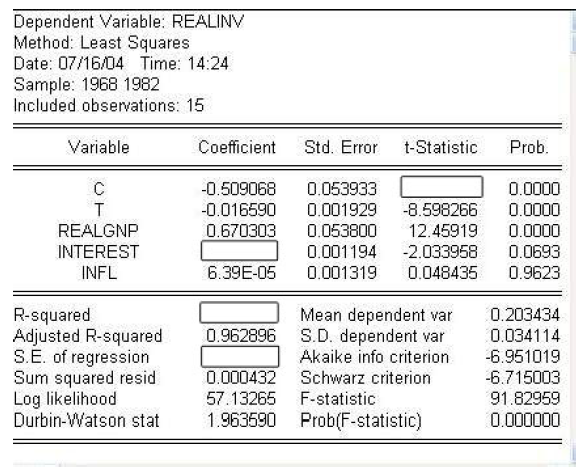
\includegraphics[width = 0.5\columnwidth]{Code1/Eviews}
\end{figure}

\section*{\underline{Exercise h}}
Assume that the data-generating process is given by
\[
y_i = \alpha + \beta_1x_{1,i} + \beta_2x_{2,i} + u_i\text{ .}
\]Consider further the wrongly specified process
\[
y_i = \alpha' + \beta'_1x_{1,i} + u'_i\text{ .}
\]The OLS estimator $\hat{\beta}'_1$ of the wrong model is given by
\[
\hat{\beta}'_1 = \hat{\beta}_1 + \hat{\beta}_2\frac{S_{x_1x_2}}{S_{x_1x_1}}\text{ .}
\]
\begin{enumerate}[label = \alph*)]
	\item Interpret the OLS estimator $\hat{\beta}'_1$. Is it unbiased?
	\item Find the OLS estimator $\hat{\alpha}'$.
	\item Interpret the equation $u_i' = \beta_2x_{2,i} + u_i$ and find the expectation of $u'_i$.
	\item Find the variance of $\hat{\beta}'_1$. Is the estimator $\hat{\sigma}^2=\frac{1}{n-k}S_{\hat{u}'\hat{u}'}$ of the wrongly specified model unbiased?
\end{enumerate}

\newpage
\section*{\underline{Exercise i}}
Consider the table below. The milk production ($m$) of a cow is a function of the fed fodder ($f$). Construct a Regression Specification Error Test ({RESET}) on a linear relationship. Let $S_{\hat{u}\hat{u}}' = 2786870$ be the sum of squared residuals of the linear specification model, while $S_{\hat{u}\hat{u}}* = 932014,3$ is the sum of squared residuals of an extended specification containing terms up to the third power. Can you reject the null hypothesis of a linear relationship?
\begin{table}[H]
	\centering
	\begin{tabular}{c|cccccccccccc}
		\toprule
		$t$ & 1&2&3&4&5&6&7&8&9&10&11&12\\
		$f$&10&30&20&33&5&22&8&14&25&1&17&28\\
		$m$&6525&8437&8019&8255&5335&7236&5821&7531&8320&4336&7225&8112\\
		\bottomrule
	\end{tabular}
\end{table}



\section*{\underline{Exercise k}}
Consider the following table:
\begin{table}[H]
	\centering
	\scriptsize
	\begin{tabular}{c|cccccccccccc}
		\toprule
		$i$ &1&2&3&4&5&6&7&8&9&10&11&12\\
		\midrule
		$x$ &10&30&20&33&5&22&8&14&25&1&17&28\\
		$y$ &2'430&19'182&10'092&22'513&1'692&12'718&2'440&3'149&10'619&1'011&6'992&17'672\\
		\bottomrule
	\end{tabular}
\end{table}	

\begin{enumerate}[label = \alph*)]
	\item You are not sure whether the relationship between $y$ and $x$ is linear. Conduct a Regression Specification Error Test on linearity. A first calculation yields $S_{\hat{u}\hat{u}} = 64.777$ and $S_{\hat{u}\hat{u}}* = 19.399$ as the sum of squared residuals of the linear model and the sxtended specification with $L=3$ respectively.
	\item The provider of the data tells you that the dependency is exponential, i.e.
	\[
	\ln(y_i) = \alpha + \beta x_i + u_i, \qquad u_i\sim\mathcal{N}(0, \sigma^2)\text{ .}
	\]Estimate $\alpha$ and $\beta$.
	\item Find the 5\%-confidence intervals for $\alpha$ and $\beta$.
	\item Find the $R^2$.
	\item The observation of $y_{13}$ for the given value $x_{13} = 15$ got lost. Find the 95\% forecasting interval for $y_{13}$.
	\item Reconsider the parts b) to e). What can you say about the estimates and intervals, if you erroneously assume that the model is linear?
\end{enumerate}

\section*{\underline{Exercise l}}
The following data, provided by \textit{Statistisches Bundesamt}, displays the economic growth rate $x_i$ and the change in the unemployment rate $y_i$ over the years 1992-2009 (in percent).
\begin{table}[H]
	\centering
	\scriptsize
	\begin{tabular}{ccccccccccccccccccc}
		\toprule
		year $i$& 92&93&94&95&96&97&98&99&00&01&02&03&04&05&06&07&08&09\\
		\midrule
		$x_i$&2.2&0.8&2.7&1.9&1.0&1.8&2.0&2.0&3.2&1.2&0.0&-0.2&1.2&0.8&3.4&2.7&1.0&-4.7\\
		$y_i$&0.9&1.3&0.6&-0.2&0.7&0.6&-0.2&-0.8&-0.8&0.1&0.8&0.9&0.5&0.9&-0.8&-1.5&-1.1&0.2\\
		\bottomrule
	\end{tabular}
\end{table}
\begin{enumerate}[label = \alph*)]
	\item This data is used to discuss the consequences of the violation of the classical assumption A3. What are the consequences and how can you solve the problem?
	\item Assume that there is a structural break between 2004 and 2005. Find an appropriate model to estimate its parameters.
	\item Is there a significant difference between the two phases?
\end{enumerate}

\section*{\underline{Exercise m}}
Consider a regression model $y_i = \alpha + \beta x_i + u_i$. The parameters are estimated by OLS and the following sums are obtained:
\[
\sum_{i = 1}^{15}{y_i} = 63.8808 \qquad \sum_{i = 1}^{15}{y_i^2} = 289.9335 \qquad \sum_{i = 1}^{15}{\hat{y}_i^2} = 272.1864
\]
\begin{enumerate}[label = \alph*)]
	\item Calculate the adjusted coefficient of determination
	\[
	\bar{R}^2 = 1 - \frac{\frac{1}{n-p-1} \sum_{i = 1}^n{(y_i - \hat{y}_i)^2}}{\frac{1}{n-1} \sum_{i = 1}^n{(y_i - \bar{y})^2}}
	\]
	\item The observations are displayed in the figure below. How do you explain the results in a)?
	\begin{figure}[H]
		\centering
		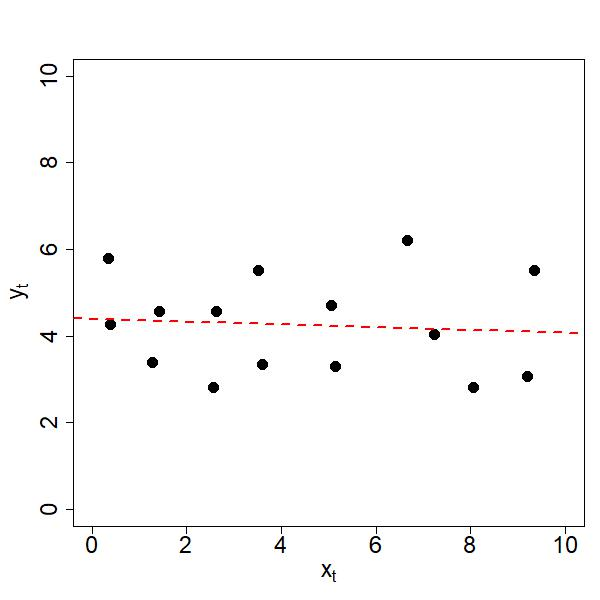
\includegraphics[width = 0.5\columnwidth]{Code1/negR.jpeg}
	\end{figure}
\end{enumerate}


The following table displays the results of a study with allergy patients. We investigate the effect of medication by assuming the model $y_i = \alpha + \beta x_i + u_i$. 
\begin{figure}[H]
	\begin{minipage}{0.5 \columnwidth}
		\begin{tabular}{cccc}
			\toprule
			\toprule
			&Dosage $x_i$ & Days of Relief $y_i$&$x_iy_i$\\
			\midrule
			&3&9&27\\
			&3&5&15\\
			&4&12&48\\
			&5&9&45\\
			&6&14&84\\
			&6&16&96\\
			&7&22&154\\
			&8&18&144\\
			&8&24&192\\
			&9&22&198\\
			\midrule
			$\Sigma$&59&151&1003\\
			SSQ&389&2651&--\\
			\bottomrule
			\bottomrule
		\end{tabular}
	\end{minipage}
	\hfill
	\begin{minipage}{0.5\columnwidth}
		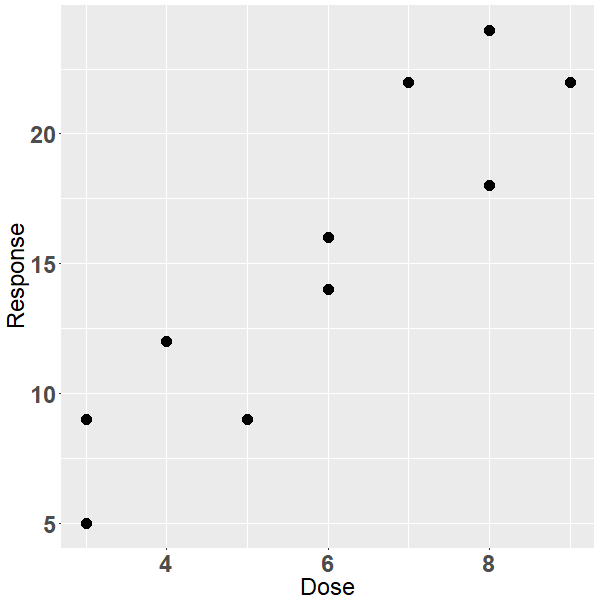
\includegraphics[width = \columnwidth]{Code1/DoseResp.png}
	\end{minipage}
\end{figure}
\begin{enumerate}[label = \alph*)]
	\item Are the assumptions satisfied?
	\item Estimate the parameters $\alpha$ and $\beta$ by OLS.
	\item Calculate the confidence intervals for $\hat{\alpha}$ and $\hat{\beta}$ and interpret.
	\item The following figure shows the 95\% confidence interval around the regression line. Try to think of a reason why the this confidence band is wider at the edges.
	\begin{figure}[h!]
		\centering
		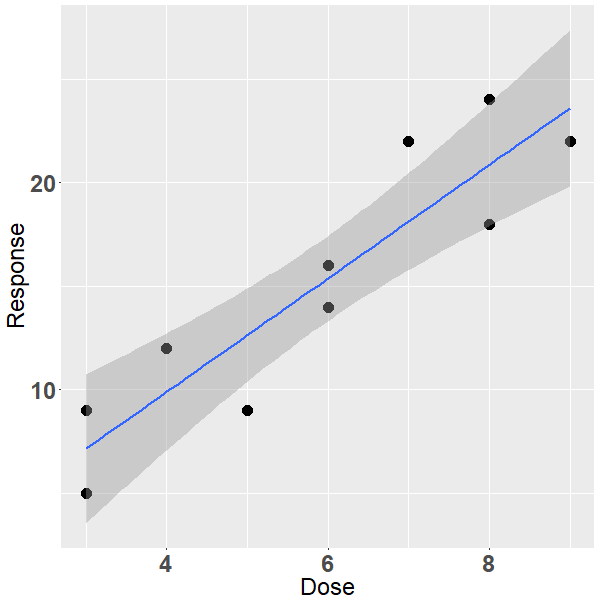
\includegraphics[width = 0.5\columnwidth]{Code1/DoseRespFit.png}
	\end{figure}
\end{enumerate}

\section*{\underline{Exercise q}}
Consider the regression model $y_i = \alpha + \beta x_i + u_i$. We are going to prove that
\[T_{\beta} = \frac{\hat{\beta} - \textrm{E}(\hat{\beta})}{\sqrt{\widehat{\textrm{Var}}(\hat{\beta})}} \sim t_{n-2}\qquad \text{and}\qquad T_{\alpha} = \frac{\hat{\alpha} - \textrm{E}(\hat{\alpha})}{\sqrt{\widehat{\textrm{Var}}(\hat{\alpha})}} \sim t_{n-2}\]
by following the steps below. It is noted that it suffices to show the left statement, in the proof for $T_{\alpha}$ the same arguments are used.
\begin{enumerate}[label = \arabic*)]
	\item Rewrite $T_{\beta}$, so that the numerator is $\mathcal{N}(0,1)$ distributed.\\
	Hint: A random variable $X\sim\mathcal{N}(\textrm{E}(X), \textrm{Var}(X))$ is standardized by subtracting its expectation and dividing by the \underline{known} standard deviation, i.e. $\frac{X-\textrm{E}(X)}{\sqrt{\textrm{Var}(X)}}\sim \mathcal{N}(0,1)$
	\item Show that the resulting denominator has a representation
	\[c\cdot\frac{\sum_{i = 1}^N{\hat{u}_i^2}}{\sigma^2} = c\cdot\sum_{i = 1}^N{\left(\frac{\hat{u}_i}{\sigma}\right)^2}\]for a constant $c$.
	\item ...?
\end{enumerate}
\end{document}